% 1- introduzione alla sezione
% 2- ragionamento sul funzionamento ipotetico del pdca e degli obiettivi di miglioramento
% 3- introduzione alla valutazione critica (andamento miglioramenti e cambiamenti nelle appendici B e C)
% 4- valutazione critica dei processi che hanno subito miglioramenti (Configurazione, Organizzazione, Pianificazione (comprendente i ruoli))
% 5- obiettivi di miglioramento di fatto raggiunti

\section{Considerazioni finali sul miglioramento}
	In questa sezione vengono riportate alcune valutazioni fatte in seguito ad un'analisi retrospettiva di tutto il lavoro svolto dall'inizio del progetto. In particolare sono stati fatti dei ragionamenti critici riguardo i miglioramenti sperimentati nei diversi processi istanziati, in modo da comprendere meglio quale sia stata l'evoluzione del \textit{way of working} e quali benefici ne ha tratto il gruppo.
	
	\subsection{Analisi critica della pratica seguita}
		Il modo migliore per garantire l'efficacia a lungo termine dei miglioramenti è applicare il ciclo PDCA, basandolo su specifici obiettivi di avanzamento quantificabili, relativi agli aspetti dei singoli processi di maggior rilevanza ai fini del progetto. Questo approccio permette di attuare dei miglioramenti proattivi, che puntino a potenziare le buone prassi già fissate, prima dell'insorgere di problematiche che necessiterebbero correzioni reattive, realizzando quindi un miglioramento continuo.
		\newline
		Durante i mesi di progetto, però, questo approccio non è stato seguito a causa dell'inesperienza del gruppo che non ha permesso di capirne pienamente l'utilità; invece, sono state spesso privilegiate azioni correttive, adottate in risposta agli errori riscontrati durante l'avanzamento del progetto. Quest'ultime, sebbene spesso tardive ed meno efficaci in ottica di miglioramento continuo, hanno il vantaggio di portare costi inferiori, in termini di risorse, rispetto alle azioni proattive.
		\newline
		Per poter applicare il ciclo PDCA, gli obiettivi di miglioramento devono essere selettivi, ossia intervenire su specifici aspetti dei processi, e misurabili, in modo da capire se e quando il loro scopo viene raggiunto. Vanno quindi scelti oculatamente, valutando opportunamente il rapporto costi/benefici, per fare in modo che il piano di miglioramento continuo sia sostenibile in base alle risorse disponibili.
	
	\subsection{Valutazioni generali sui miglioramenti}
		\begin{figure}[H]
			\centering
			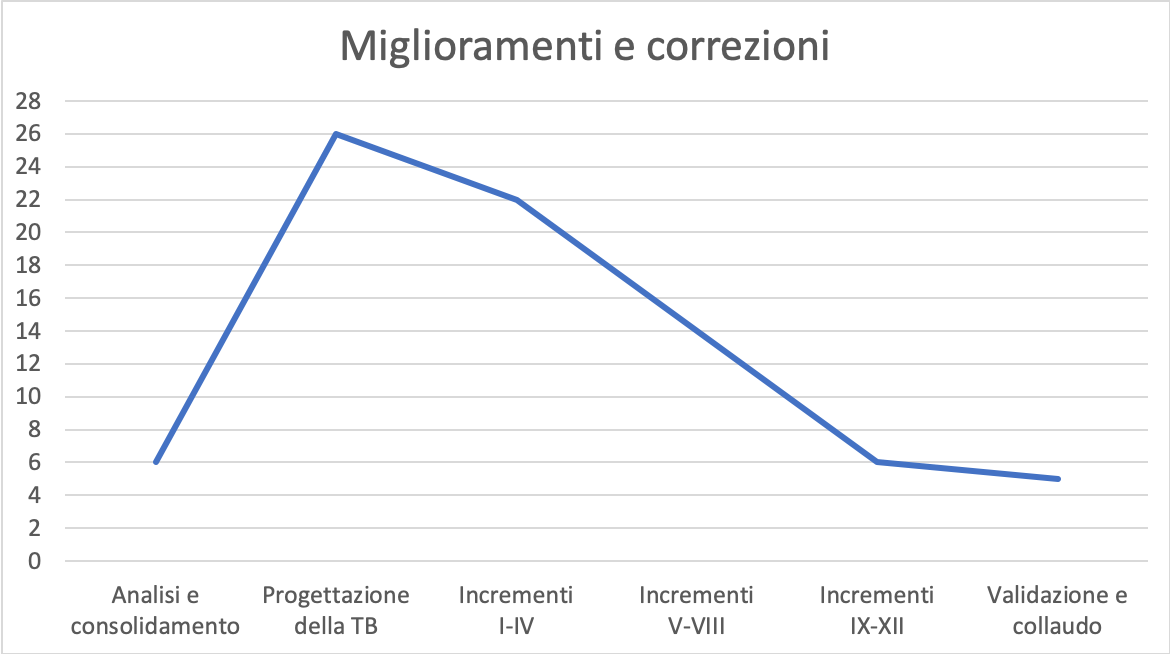
\includegraphics[width=1.0\linewidth]{./res/images/miglioramenti.png}
			\caption{Andamento del numero di miglioramenti e correzioni nelle diverse fasi del progetto}
			\label{fig:Andamento del numero di miglioramenti e correzioni nelle diverse fasi del progetto}
		\end{figure}
	
		Nonostante non siano stati posti specifici obiettivi e siano state applicate principalmente azioni correttive, durante lo sviluppo del progetto è stato comunque possibile apprezzare alcuni miglioramenti a specifiche attività dei processi che compongono il \textit{way of working} del gruppo. Come mostra il grafico \ref{fig:Andamento del numero di miglioramenti e correzioni nelle diverse fasi del progetto}, il numero di valutazioni di miglioramento e cambiamenti era inizialmente molto basso; questo a causa dell'inesperienza e della mancanza di capacità autocritica del gruppo nelle prime settimane, nelle quali, oltretutto, il \textit{way of working} del team era ancora in fase di definizione. Tale numero è poi cresciuto molto nelle fasi successive, sia a causa di una maggior esperienza e familiarità con le attività da svolgere, che ha permesso uno sguardo critico sul modo in cui erano eseguite, sia per le osservazioni puntuali ricevute dai committenti. La curva risulta poi sempre discendente, ad indicare un progressivo raffinamento del metodo di lavoro del gruppo, che ha portato ad aver sempre meno bisogno di miglioramenti: il lavoro svolto ha quindi portato dei benefici non solo ai prodotti, ma anche ai processi.
	
	\subsection{Valutazioni specifiche sui miglioramenti nei processi}
		Di seguito vengono riportate delle valutazioni critiche atte ad indicare quali miglioramenti sono stati rilevati nelle attività di alcuni dei processi istanziati dal gruppo. Per ogni attività analizzata saranno riportati gli specifici obiettivi di miglioramento raggiunti nel corso del progetto.	Tali obiettivi, frutto di un'analisi retrospettiva sul lavoro svolto, sono stati individuati nella fase finale del progetto.
	
		\subsubsection{Gestione dei processi}
			\paragraph{Gestione delle comunicazioni e degli incontri}
				Tra le attività a cui sono state apportate più migliorie nel corso del progetto ci sono la gestione delle comunicazioni e la gestione degli incontri.
				\newline
				Nelle prime settimane il gruppo si riuniva spesso e in incontri molto lunghi, perché era necessario conoscersi, oltre che decidere molti dettagli del metodo di lavoro e delle attività da svolgere. Nelle fasi centrali del progetto queste esigenze si sono ridotte, e quando, a causa dell'emergenza sanitaria, il team non ha più potuto riunirsi di presenza, tutti i membri sono stati in grado di adattarsi alla situazione senza che questo causasse rallentamenti allo sviluppo. Il gruppo si è impegnato a sfruttare al massimo le potenzialità degli strumenti di comunicazione in uso; è stata regolarizzata la frequenza degli incontri e la loro durata è stata limitata al necessario per risolvere dubbi e prendere decisioni, aspetto molto più difficile da controllare negli incontri di presenza.
				\newline
				In generale, tutti gli elementi del gruppo hanno garantito la propria reperibilità: ciò ha permesso di risolvere rapidamente problemi ed incomprensioni e di non rimandare decisioni collettive. In questo modo, nonostante lavorare a distanza rischiasse di danneggiare le comunicazioni interne, il gruppo è riuscito a mantenere costante il ritmo di lavoro e a sfruttare meglio il tempo. In modo analogo sono stati gestiti anche i rapporti con i committenti grazie a videoconferenze e scambio di mail il rapporto non ha risentito della mancanza di incontri di persona.
				
				\subparagraph{Obiettivi di miglioramento raggiunti}
					Nelle attività di gestione delle comunicazioni e degli incontri sono stati raggiunti i seguenti obiettivi di miglioramento:
					\begin{itemize}
						\item ridurre la durata degli incontri ordinari (schedulati periodicamente) ad un massimo di 1 ora per ridurre gli sprechi di tempo ed aumentare la produttività.
					\end{itemize}
		
			\paragraph{Pianificazione}
				Modifiche e miglioramenti sono stati apportati in larga misura anche a tutto ciò che riguardava l'attività di Pianificazione: sia ai ruoli di progetto che alla effettiva pianificazione del lavoro del gruppo.
				\newline
				Nonostante fosse noto sin dall'inizio cosa spettasse ai diversi ruoli, addentrandosi nel progetto è stato necessario rispondere con prontezza alle nuove attività da svolgere, assegnandole al ruolo giusto; inoltre, l'emergenza sanitaria ha costretto il \textit{Responsabile} e l'\textit{Amministratore} a riorganizzare risorse e strumenti in modo da fronteggiare al meglio la situazione. Anche il ruolo di \textit{Verificatore} si è evoluto, soprattutto grazie all'esperienza accumulata nei mesi e al supporto di strumenti di verifica adatti.
				\newline
				Su segnalazione dei committenti, il gruppo ha più volte rivisto la struttura della propria pianificazione di progetto. Il primo cambiamento ha riguardato la divisione degli obiettivi di sviluppo in incrementi, e la riorganizzazione della pianificazione in funzione di questa modifica: ad ogni incremento è stato assegnato un periodo, le attività e il monte ore necessari al raggiungimento degli obiettivi. La divisione dei requisiti in gruppi piccoli ha aiutato il gruppo a focalizzarsi sullo sviluppo di un ristretto numero di funzionalità alla volta, senza dispersione di energie; la scansione degli incrementi ha anche permesso di regolarizzare le attività di verifica e rilevazione delle metriche su processi e prodotti. Tuttavia, poiché questa divisione troppo minuta rischiava di frammentare lo sviluppo e di far perdere la visione complessiva del prodotto a livello di obiettivi di avanzamento, gli incrementi sono stati poi raggruppati in più fasi: in questo modo si sono avute sia la visione di dettaglio che quella di più ampio respiro.
				
				\subparagraph{Obiettivi di miglioramento raggiunti}
					Nell'attività di pianificazione sono stati raggiunti i seguenti obiettivi di miglioramento:
					\begin{itemize}
						\item ridurre la durata delle fasi ad un massimo di 14 giorni per poterne monitorare meglio l'uso delle risorse.
					\end{itemize}
		
		\subsubsection{Gestione della configurazione}
			Per il processo di gestione della configurazione, il gruppo ha lavorato maggiormente su tre aspetti: lo schema di versione, l'automazione dei workflow con \textit{continuous integration} e l'automazione dell'installazione e dell'aggiornamento del sistema in rete.
			
			\paragraph{Versionamento e rilascio}
				Il numero di versione assegnato secondo lo schema iniziale non dava alcuna garanzia rispetto ad aggiunte o modifiche al prodotto non verificate, quindi potenzialmente sbagliate. Questo problema è stato risolto permettendo uno scatto di versione ad ogni modifica o aggiunta \textbf{debitamente verificata e approvata}. Contestualmente, è stata fissata anche una notazione che legasse la versione alla pianificazione per incrementi: questa ulteriore scansione del numero di versione per obiettivi di sviluppo (quelli degli incrementi) permetteva inoltre di unificare la versione di prodotti software e documentali. L'ultimo perfezionamento allo schema di versione ha visto il passaggio ad un sistema basato a quello semantico, per cui lo scatto di versione è determinato dall'impatto delle modifiche sul contenuto del prodotto già presente.
				\newline
				Poiché il sistema sviluppato è articolato in più componenti indipendenti, il suo avvio richiederebbe l'esecuzione manuale di diverse azioni di installazione, compilazione e lancio, una per ciascun componente. Il gruppo ha allora prodotto uno script unico che raccolga tutti questi comandi: scarica i sorgenti aggiornati da tutti i submodules del repository, se non già presenti in locale, ed esegue gli step di compilazione ed esecuzione individuale delle varie parti. In questo modo è possibile installare, aggiornare ed avviare il sistema con un singolo comando (il lancio dello script), rendendo la procedura più agile e veloce in ottica sia di sviluppo e test che di messa in produzione dei nuovi rilasci.
				
				\subparagraph{Obiettivi di miglioramento raggiunti}
					Nelle attività di versionamento e rilascio sono stati raggiunti i seguenti obiettivi di miglioramento:
					\begin{itemize}
						\item ridurre ad 1 il numero di azioni manuali necessarie per installare il prodotto;
						\item ridurre ad un massimo di 10 minuti il tempo di installazione e avvio del prodotto.
					\end{itemize}
			
			\paragraph{Continuous integration, notification e monitoring}
				Passando agli strumenti per la verifica, l'implementazione della \textit{continuous integration} tramite GitHub Actions ha permesso di innescarne l'attivazione ad ogni push relativo al submodule cui essa riferiva; questa prassi garantiva un monitoraggio costante dello stato del prodotto software. Inoltre, un controllo automatico impediva l'aggiunta di nuovo codice nel submodule se questo non completava con successo tutti i controlli previsti; in questo modo si assicurava la presenza di una versione verificata e funzionante del prodotto software all'interno del repository. Infine, l'uso di un \textit{webhook} ha permesso di collegare la CI ad un bot di Slack, in modo che tutti i membri del gruppo venissero prontamente informati, tramite notifica, ad ogni fallimento della \textit{continuous integration} nei vari submodules del repository del progetto.
				
				\subparagraph{Obiettivi di miglioramento raggiunti}
					Nelle attività di continuous integration, notification e monitoring sono stati raggiunti i seguenti obiettivi di miglioramento:
					\begin{itemize}
						\item aumentare la frequenza settimanale di esecuzione di controlli di CI ad un minimo di 20 per rilevare tempestivamente gli errori introdotti.
					\end{itemize}

